% Created 2021-08-05 Thu 18:09
% Intended LaTeX compiler: pdflatex
\documentclass[11pt]{article}
\usepackage[utf8]{inputenc}
\usepackage[T1]{fontenc}
\usepackage{graphicx}
\usepackage{grffile}
\usepackage{longtable}
\usepackage{wrapfig}
\usepackage{rotating}
\usepackage[normalem]{ulem}
\usepackage{amsmath}
\usepackage{textcomp}
\usepackage{amssymb}
\usepackage{capt-of}
\usepackage{hyperref}
\usepackage[letterpaper, portrait, margin=1in]{geometry}
\author{Piero Panariello}
\author{Piero Panariello}
\date{\today}
\title{Developer Documentation for Mathcad Automation Software\\\medskip
\large Thornton and Tomasetti}
\hypersetup{
 pdfauthor={Piero Panariello},
 pdftitle={Developer Documentation for Mathcad Automation Software},
 pdfkeywords={},
 pdfsubject={},
 pdfcreator={Emacs 27.2 (Org mode 9.4.4)}, 
 pdflang={English}}
\begin{document}

\maketitle
\tableofcontents


\section{Technologies Used}
\label{sec:orgce4091d}
\begin{enumerate}
\item Python is the programming language of choice
\item PySimpleGUI : used to render the graphical user interface. \href{https://pysimplegui.readthedocs.io/en/latest/}{Documentation}
\item MathcadPy : wrapper written in python used to access the Mathcad api. \href{https://github.com/MattWoodhead/MathcadPy/blob/master/MathcadPy/\_application.py}{Documentation}
\item Openpyxl : used to interface with the excel documents.\href{https://openpyxl.readthedocs.io/en/stable/}{ Documentation}
\item PyInstaller: used to freeze the python program into an executable.\href{https://pyinstaller.readthedocs.io/en/stable/}{ Documentation}
\item Look in \textasciitilde{}./dist/requirements.txt to view all the dependencies
\item Look in \textasciitilde{}./dist/info.txt for more information on how to package the application and how to re-create the python virutal environment.
\end{enumerate}

\section{File Descriptions}
\label{sec:org3997b83}
All files are located in the ./dist directory. 
\begin{enumerate}
\item \textbf{info.txt}
\begin{itemize}
\item This file has information about how to re-create the development environment and how to package and distribute the application. Consult the section \textbf{Packaging and Distribtion} for more information.
\end{itemize}
\item \textbf{img\_to\_b64.py}
\begin{itemize}
\item In order to allow images to be displayed within the application, we cannot use traditional .jpg or .png files. We must convert them to a binary format. This allows images to be stored as strings (base64 format). This file converts .png and .jpg files into a python file containing string variables. These variables hold the information of those photos in base46 format. Run the script using \textbf{python img\_to\_b64.py}.
\end{itemize}
\item \textbf{images.py}
\begin{itemize}
\item This file holds the images we will be using in the application as python variables in base64 format.
\end{itemize}
\item \textbf{main.py}
\begin{itemize}
\item The application source code. Ensure the developer environment is activated and run \textbf{python main.py} to start the application.
\end{itemize}
\item \textbf{requirements.txt}
\begin{itemize}
\item Holds the name and versions of all the python packages that the program uses. You will use this file when creating the developer environment. Read more in the \textbf{Re-Creating the Virtual Environment} section.
\end{itemize}
\item \textbf{./main\_build/MathcadPy}
\begin{itemize}
\item This is the python wrapper for Mathcad. It is directly imported in to the application. Feel free to edit this file if the connection to the API is not working for some reason.
\end{itemize}
\item \textbf{./main\_build/dependencies}
\begin{itemize}
\item All of the dependencies that the program uses are located here.
\item \textbf{data.py}
\begin{itemize}
\item Holds the Equipment and Output Classes. Modify this file to change the classes
\end{itemize}
\item \textbf{filestream.py}
\begin{itemize}
\item Handles any operation that deals with files on the hard disk. For example, reading from the excel input file, writing to the csv, and saving to the excel input file.
\end{itemize}
\item \textbf{gui.py}
\begin{itemize}
\item All of the GUI (graphical user interface) elements that are not the main window (main.py) are declared here. This includes popup windows and the choose file window you see at startup.
\end{itemize}
\item \textbf{helpers.py}
\begin{itemize}
\item Holds all helper functions the program needs. Ex: \textbf{gen\_random\_string(length:int)->str}
\end{itemize}
\item \textbf{reports.py}
\begin{itemize}
\item Anything having to do with generating reports or mathcad calculations takes place in this file.
\end{itemize}
\item \textbf{validation.py}
\begin{itemize}
\item Validates inputs given by the user. Ensures proper inputs are given, and will throw error if not.
\end{itemize}
\item \textbf{verbose.py}
\begin{itemize}
\item Handles converting strings like w\_p\_input into a more readable format. Handles converting inputs and outputs into a more verbose format.
\end{itemize}
\end{itemize}
\end{enumerate}

\section{Mathcad API}
\label{sec:org70ebe8f}
Currently, the Mathcad API supports Mathcad Prime 3.0 and above. From my testing it works best with Mathcad Prime 7.0 (the lastest version). The API documentation can be located \href{https://support.ptc.com/help/mathcad/r7.0/en/index.html\#page/PTC\_Mathcad\_Help\%2Fmathcad\_and\_automation\_api.html\%23}{here}. You can purchase the SDK from Mathcad to get more information and examples, but I would recommend against it (it's \$9000).
\section{Datypes and Storage of Data}
\label{sec:orgf8c7d8f}
\subsubsection{Equipment Class: (stores all the equipment from the excel file)}
\label{sec:org08cddcd}
\begin{enumerate}
\item Class variables:
\label{sec:orga99ecc8}
\begin{itemize}
\item \textbf{self.items} = list()
\end{itemize}
List of all the equipment in the excel file, stored as individual dictionaries.

\begin{itemize}
\item \textbf{self.cur\_index} = 0
\end{itemize}
The current index of the equipment that the user is viewing in the GUI

\begin{itemize}
\item \textbf{self.length} = 0
\end{itemize}
Holds the length of self.items

\begin{itemize}
\item \textbf{self.fields} = list()
\end{itemize}
A list of all the elements from the header row from the excel document

\begin{itemize}
\item \textbf{self.names} = list()
\end{itemize}
A list of all the equipment names from the excel document

\begin{itemize}
\item \textbf{self.inputs} = list()
\end{itemize}
A list of all the inputs from the header row in the excel document

\begin{itemize}
\item \textbf{self.outputs} = list()
\end{itemize}
A list of all the outputs per equipment generated when the user clicked \textbf{Preview Calculation Outputs}. 

\item Class methods:
\label{sec:org2cb4996}

\begin{itemize}
\item \textbf{append(self, to\_append:dict)} Takes in a dict as an argument
\end{itemize}
Appends self.items with the new equipment dictionary, appends self.names, appends self.inputs

\begin{itemize}
\item \textbf{next\_index(self)} No arguments
\end{itemize}
Increments the value of self.cur\_index

\begin{itemize}
\item \textbf{prev\_index(self)} No arguments
\end{itemize}
Decriments the value of self.cur\_index
\end{enumerate}

\subsubsection{Outputs Class: (stores the values of the outputs when the user decides to preview the output variables from the Mathcad file)}
\label{sec:org5c6964b}
\begin{enumerate}
\item Class variables:
\label{sec:org7016954}

\begin{itemize}
\item \textbf{self.items} = list()
\end{itemize}
Follows the format:
\begin{verbatim}
# alias, [value, unit, power]
['f_p_max_output', [408.81554560308007, 'kg', 0]],
['f_p_min_output', [76.65291480057748, 'kg', 0]],
['f_p_tot_output', [76.65291480057748, 'kg', 0]],
...
\end{verbatim}
\item Class methods:
\label{sec:org2cd14dd}
\begin{itemize}
\item \textbf{append(self, to\_append)} Takes tuple or list argument
\end{itemize}
Converts to\_append to array and appends self.items

\begin{itemize}
\item \textbf{clear(self)} Takes no arguments
\end{itemize}
Clears self.items

\begin{itemize}
\item \textbf{display(self)->list} Takes no arguments
\end{itemize}
Returns a list of variables and values that is easier to display in the GUI. Makes outputs verbose so they are easier to read. Rounds decimals to 2 digits. 
Ex: [ 'f\_p\_tot\_output = 408.82 kg', 'f\_p\_min\_output = 76.65 kg', \ldots{}]
\end{enumerate}

\section{API Details}
\label{sec:org8fa64e6}

The MathcadPy library is used as a wrapper that allows you to access all of the mathcad api endpoints from the comfort of Python. You can read more about the Mathcad API \href{https://support.ptc.com/help/mathcad/r7.0/en/index.html\#page/PTC\_Mathcad\_Help\%2Fmathcad\_and\_automation\_api.html\%23}{here}. The API allows you to modify and change Mathcad Prime files. Despite PTC's documenation, you cannot print documents.

\textbf{get\_eqpt\_from\_xl(filepath:str)->Equipment}
\begin{itemize}
\item located in ./dist/main\_build/dependencies/filestream.py
Takes in the filepath of the input excel file and returns the \textbf{Equipment} object. This function is executed right after the choose files window is closed.

The excel table looks similar to the one below:
\begin{center}
\begin{tabular}{llrll}
\hline
eqpt\_name & mounting\_location & project\_number & tags & eqpt\_tags\\
\hline
Anesthesia machine & Wall, Floor & 1111 & Medical, ICU, something & Foo, Bar\\
Warming Cabinet & Floor & 1111 & Medical & Foo, Bar\\
Surgical Scrub Sink & Wall & 1111 & Medical & Foo, Bar\\
Retratable Ceiling Column & Ceiling & 1111 & Medical & Foo, Bar\\
\hline
\end{tabular}
\end{center}
\end{itemize}

\textbf{pre\_generate\_report(equipment:Equipment, files, generating\_multiple\_reports = False)}
\begin{itemize}
\item located in ./dist/main\_build/dependencies/reports.py
This acts as a pre-fight test. It checks if the proper template is given for the equipment and passes the equipment and a uniquely generated filename to the generate\_report function.
\end{itemize}

\textbf{generate\_report(cur\_eqpt, equipment:Equipment, file\_name:str, template\_file:str, files, debug = False)->bool}
\begin{itemize}
\item located in ./dist/main\_build/dependencies/reports.py
The function connects to the Mathcad API, opens the template file specific to the mounting location, updates the input values specific to the equipment, and then saves the document. If generateing multiple reports, multithreading is used to speed up the process. Currently 4 threads are being used, but feel free to increase this number if the workflow demands more throughput. This variable is called \textbf{num\_threads} in the event \textbf{generate\_report\_for\_all}. (Events are how PySimpleGUI handles buttons being pressed. Events are checked in the main GUI loop.)
\end{itemize}

\textbf{mathcad\_calculate(eqpt, files, debug = False)->dict}
\begin{itemize}
\item located in ./dist/main\_build/dependencies/reports.py
Allows the user to preview the Mathcad calculation output. It duplicates the template file into a temp file, takes the inputs and waits for the outputs to generate. It then deletes the temp file when finished. It returns a dictionary with the output values. The debug variable changes if Mathcad will display the windows being edited or not. When \textbf{debug = False}, no window is shown, when \textbf{debug = True}, windows are shown.
\end{itemize}

\textbf{def save\_eqpt\_to\_xl(equipment: Equipment, filepath:str)->bool}
\begin{itemize}
\item located in ./dist/main\_build/dependencies/filestream.py
Saves the inputs the user has changed in the application back to the excel file. Works similarly \textbf{get\_eqpt\_from\_xl} but in reverse. Cannot save to the excel file if it is open.
\end{itemize}

\section{Rendering to the GUI}
\label{sec:org83dbcfc}
\textbf{Choose equipment}
\begin{itemize}
\item Once the user has input the excel file they want to read from, the program extracts all information in the \textbf{get\_eqpt\_from\_xl} function and places all the equipment names in the Choose Equipment column.
\end{itemize}

\textbf{Inputs}
\begin{itemize}
\item Once we get the Equipment from the \textbf{get\_eqpt\_from\_xl} function, we can then render it to the input fields in the GUI.
\end{itemize}

\textbf{Outputs}
\begin{itemize}
\item If the user clicks the Preview Calculation Outputs button, the inputs from the current equipment being used is sent to the template corresponding to the correct mounting location and the output fields are gathered via the \textbf{mathcad\_calculate} function. The outputs are saved in the Outputs class, the category of the output is decided verbose.py/is\_asd\_output and verbose.py/is\_lfrd\_output, converted to verbose names, and the information is displayed in the GUI.
\end{itemize}

\textbf{Preview Images}
\begin{itemize}
\item The user has the option to include preview images that correspond to the mounting locations. The images must be included in the excel document. Use the example\_sheet.xlsx as a template. Images muse be .png or .jpg or .jpeg. The images are gathered from the excel sheet using the \textbf{get\_images\_from\_xl(self, num\_images:int)} function. Images are stored as binaries. When the user views a different equipment, the image corresponding to the mounting location is loaded into the Image Preview section of the GUI. Use ./dist/img\_to\_b64.py to convert images from .png/.jpg to binaries. It provides a python file called output.py with the binaries stored in variables. Preview images are automatically converted to binaries in \textbf{get\_images\_from\_xl}.
\end{itemize}

\section{Saving to the Database}
\label{sec:org16f41f6}
The database is a .csv file which holds some important information about generated repors. The function save\_to\_csv is used. When the user decides to save the report to the database, they are saving the equipment name, mounting location, tags, and the generated report's unique filename. The user can choose a specific database to save to, or it will save to the default database located in the \textbf{mathcad\_automation\_output} directory.

The table looks like the one below:
\begin{center}
\begin{tabular}{rllll}
\hline
Date & Tags & Name & Mounting Location & File Name\\
\hline
2021-06-30 & MEDICAL & RET\ldots{} COLUMN & CEILING & test.mcdx\\
2021-06-30 & MEDICAL & RET\ldots{} COLUMN & CEILING & Retractable\_\ldots{}.mcdx\\
2021-06-30 & MEDICAL & SUR\ldots{} SINK & WALL & Surgical\_\ldots{}.mcdx\\
\hline
\end{tabular}
\end{center}

\section{Flowchart}
\label{sec:org6611239}
\begin{figure}[htbp]
\centering
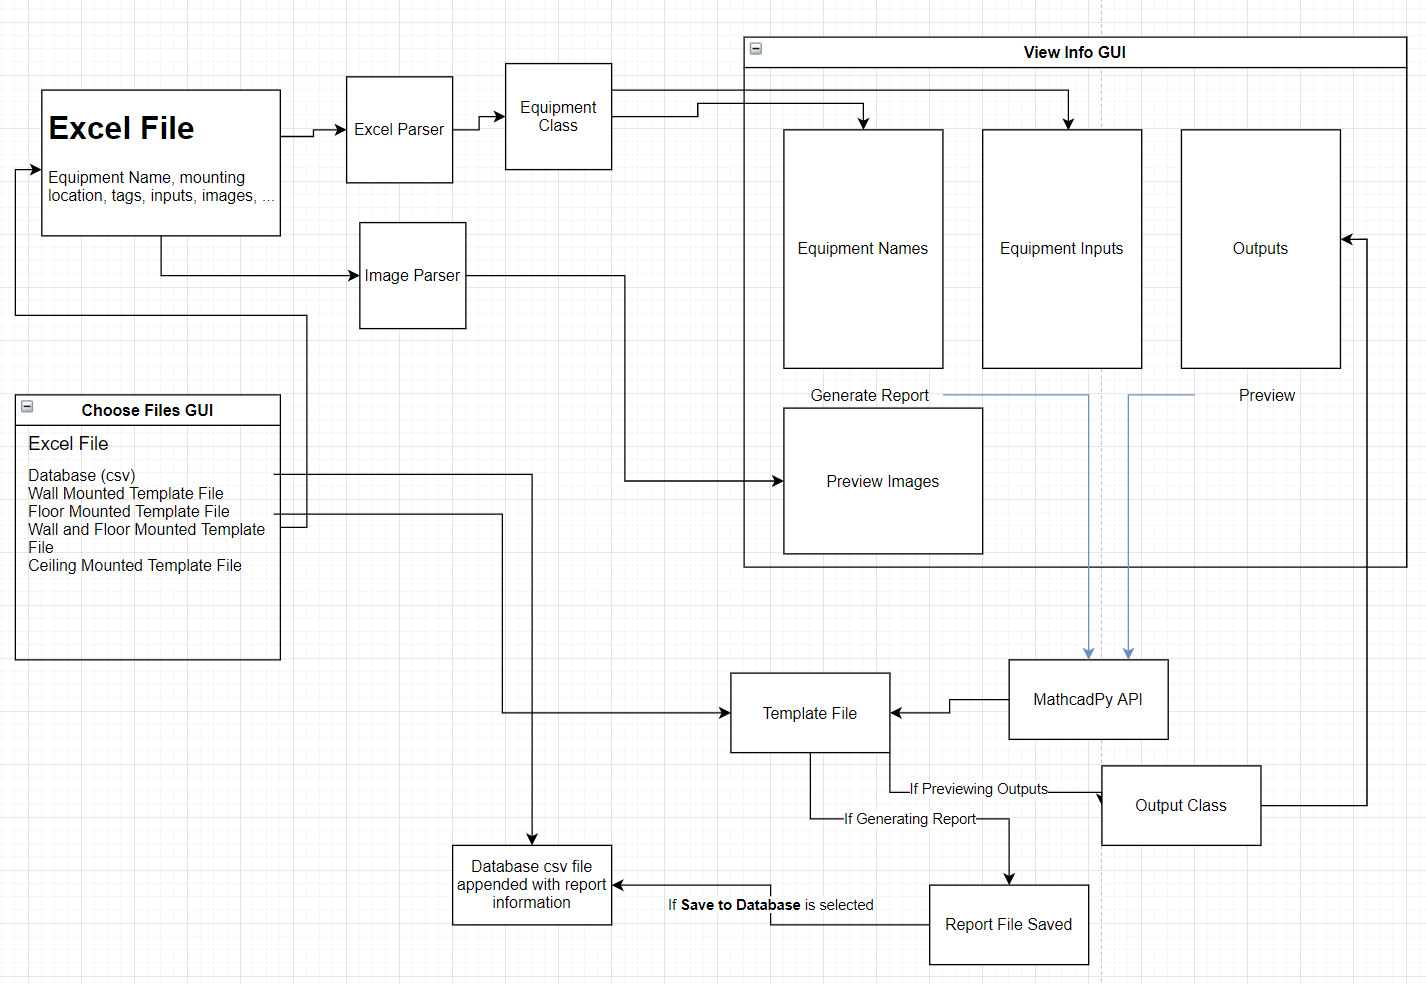
\includegraphics[width=.9\linewidth]{./dist/documentation/component_flowchart.png}
\caption{\label{fig:org3922dbb}Flow chart of program API}
\end{figure}

\section{Improving Performance}
\label{sec:org395bf22}
While the application is performant, there are a few ways to tune the application to improve performance. The function that is least performant is the \textbf{generate\_report\_for\_all} event. Multiple reports need to be generated through Mathcad. To improve performance, I implemented parallel processing. This allows multiple processes to run at the same time: each report is run on a seperate process and is then joined when each process finishes. The \textbf{num\_threads=16} variable allows you to adjust the number of parallel processes occuring. This number is limited to your computer's available threads. I suggest starting at \textbf{num\_threads = 16} and slowly increasing the variable by powers of 2 (ex: 16, 32, 64) until you achieve the desired performance. Keep in mind that the speed in which the Mathcad API can run to generate a single report is constant. Increasing \textbf{num\_threads} will only increase performance if the number of reports to be generated is greater than \textbf{num\_threads}. Note that performance will not be increased if \textbf{num\_threads} is greater than the number of reports to be generated

\section{Re-Creating the Virtual Environment}
\label{sec:orgb4bcacb}
Typical python projects use a "virtual environment" to test and develop the application. This allows for consitancy between machines running the same program. In order to activate the virtual environment, first install \textbf{virtualenv} using pip. Open PowerShell and type the following commands:

Install virtualenv 
\begin{verbatim}
pip install virtualenv
\end{verbatim}

Create the virtual environment in the project's ./dist directory
\begin{verbatim}
python -m venv env
\end{verbatim}

Activate the virtual environment
\begin{verbatim}
env\scripts\activate
\end{verbatim}

Install all the requirements into the virtual environment
\begin{verbatim}
pip install -r requirements.txt
\end{verbatim}

You can now make changes to the application in \textbf{main.py} and run the application with those new changes.

\section{Packaging and Distribution}
\label{sec:org329b412}
I have found that PyInstaller is the best method to package python applications. It "freezes" the code in order to create an executable. Install PyInstaller using pip, and ensure that it is installed by typing \textbf{PyInstaller} in PowerShell. If it is properly installed, run the code below within the activated virtual environment to package the application. Copy the following code onto one line in PowerShell and run it.
\begin{verbatim}
 PyInstaller --onefile --windowed 
--paths= "C:\Users\Owner\Desktop\mathcad_auto\dist\main_build\MathcadPy"
-i  "C:\Users\Owner\Desktop\mathcad_auto\dist\main_build\images\ma_logo.ico" 
--name "Mathcad_Anchorage_Automation_v1.1" main.py
\end{verbatim}
\end{document}
